\documentclass{article}
\usepackage[latin1]{inputenc}
\usepackage{enumerate}
\usepackage{hyperref}
\usepackage{graphics}
\usepackage{graphicx}
\usepackage{caption}
\usepackage{subcaption}
\usepackage{tabularx}
\usepackage{amsmath}
\usepackage{amssymb}
\newcommand{\ket}[1]{\ensuremath{\left|#1\right\rangle}}
\newcommand{\bra}[1]{\ensuremath{\left\langle#1\right|}}
\newcommand{\braket}[2]{\ensuremath{\left\langle #1 \middle| #2 \right\rangle}}
\newcommand{\obar}[1]{\ensuremath{\overline{ #1 }}}
\hypersetup{colorlinks=true, urlcolor=blue, linkcolor=blue, citecolor=red}
\graphicspath{ {C:/Users/Evan/Desktop/} }
\title{Determination of Magnitude and Intrinsic Flux of HD 227858 and HD 338931 from Landolt Standard SA 113475}
\author{Evan Ott \\ UT EID: eao466}
\date{\today}
\setcounter{secnumdepth}{0}
%\usepackage[parfill]{parskip}
\begin{document}
\maketitle
\section{Introduction}
While the casual astrophotographer might only care about seeing as many stars as possible in an image, in academic astronomy,
we often want to have quantifiable data about stars, for example the magnitude (measure of brightness) of the star to compare it
to others, either in terms of total light or broken into sections of the electromagnetic spectrum by filters. Or, we might want to
have the flux (photon energy or number per area each second). However, besides having proper equipment, much calibration
must take place to account for all present factors - atmospheric extinction of photons travelling at different angles
through Earth's atmosphere, ever-present and never-present pixels in sensors, absorption in mirrors and lenses, etc. Here, I work through calculating the magnitude and intrinsic flux (flux just outside the atmosphere) of stars HD 227858 (see Figure \ref{fig:hd2})
and HD 338931 (see Figure \ref{fig:hd3}) based on the Landolt Standard star SA 113475 (see Figure \ref{fig:sa})\cite{landolt}. 

\begin{figure}[h]
\centering
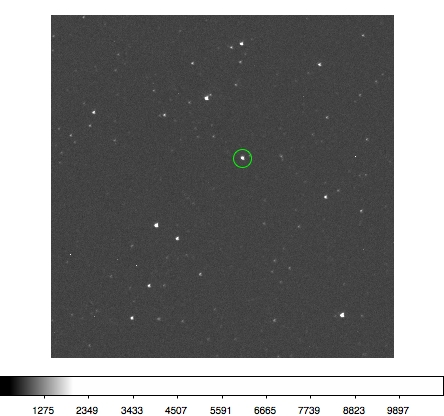
\includegraphics[scale=.75]{hd2.jpg}
\caption{\label{fig:hd2} HD 227585 and surrounding stars, colored by linear scale in number of counts per pixel.}
\end{figure}

\begin{figure}[h]
\centering
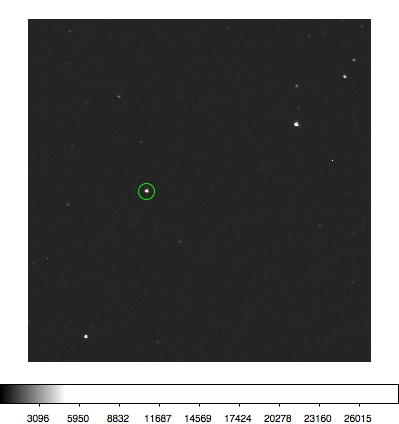
\includegraphics[scale=.75]{hd3.jpg}
\caption{\label{fig:hd3} HD 338931 and surrounding stars, colored by linear scale in number of counts per pixel.}
\end{figure}

\begin{figure}[h]
\centering
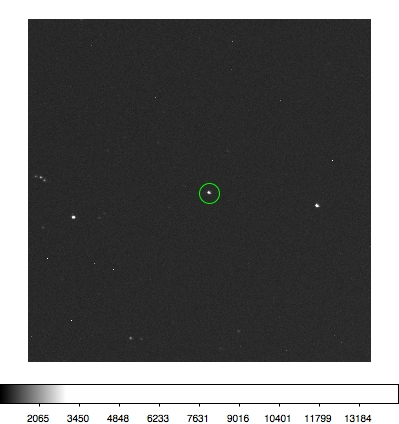
\includegraphics[scale=.75]{sa1.jpg}
\caption{\label{fig:sa} Landolt Standard star SA 113475 and surrounding stars, colored by linear scale in number of counts per pixel.}
\end{figure}

\begin{table}
\begin{center}
\begin{tabular}{c | c | c | c}
Filter & $\lambda_0$ & $\Delta\nu$ & Absolute Spectral Radiance  \\
 & [$\mu$m]& [Hz]& [erg cm$^{-2}$s$^{-1}$\AA$^{-1}$] \\
\hline
B & 0.44 & 3.06E15 & 6.60E-9 \\
V & 0.55& 3.37E15 &3.64E-9 \\
R & 0.70& 1.36E15 &1.36E-9 \\
I & 0.90& 6.81E14&8.30E-10
\end{tabular}
\end{center}
\caption{Johnson Filter Band parameters, with $\lambda_0$ as the central wavelenth,
$\Delta\nu$ as the FWHM of frequency of the filter and absolute spectral radiance as the
flux per wavelength to be observed through the filter for a 0-magnitude star in the band.}
\label{table:filters}
\end{table}

\section{Methods}
Using the 16" telescope at Robert Lee Moore Hall at the University of Texas at Austin, I and my classmates used a 1024x1024 CCD imaging
system, coupled with a selection of Johnson-type filters for the B, V, R, and I parts of the spectrum to analyse HD 227858 and HD 338931. Parameters of the filters can be found in Table
\ref{table:filters}. After taking dark frame and flat frame images (to account for the CCD's inherent background response to temperature and
non-uniform sensitivity, respectively), we were able to use the IRAF suite of programs to isolate the count (in Arbitrary Data Units [ADU])
in the image due to photons from the stars of interest and the count associated with background light from other sources. These data
are found in Table \ref{table:Counts}.

\begin{table}
\begin{center}
\begin{tabular}{c | c | c | c | c | c }
Star & Filter & t & $X=\sec{z}$ & $S_{*,sky}$ & $S_*$\\
 &  & [s]&  & $\mathsf{SUM}$ & $\mathsf{FLUX=SUM-MSKY*AREA}$\\
\hline
HD 227858 & B & 30 & 1.294 & 117809 & 39381 \\
HD 227858 & V & 30 & 1.301 & 388133 & 131079  \\
HD 227858 & R & 30 & 1.307 & 567655 & 254168  \\
HD 227858 & I &  30 & 1.323 & 417430 & 260971   \\
HD 338931 & B & 30 & 1.394 & 255793 & 152570 \\
HD 338931 & V & 30 & 1.405 & 767017 & 494401  \\
HD 338931 & R & 30 & 1.413 & 1390626 &  977589 \\
HD 338931 & I & 30 &  1.424 & 1285304 &  1075136 \\
SA 113475 & B & 30 & 1.206  & 169993 & 38822  \\
SA 113475 & B & 30 & 1.482  & 179149 &  33471 \\
SA 113475 & V & 30 & 1.207  & 477466 & 154874 \\
SA 113475 & V & 30 & 1.498  & 665531 &  147737 \\
SA 113475 & R & 30 & 1.209 & 802783  & 344417  \\
SA 113475 & R & 30 & 1.498 & 1064716 & 332641 \\
SA 113475 & I & 30 & 1.213 & 477466  & 154874  \\
SA 113475 & I & 30 & 1.521& 665531 & 147737   \\
\end{tabular}
\caption{Signal for each target star as extracted from IRAF's ${\texttt{apphot phot}}$ function, presented with
signal including background signal ($S_{*,sky}$), and signal with sky removed ($S_*$). $t$ is the exposure time in seconds,
and $X$ is the airmass given as the secant of the zenith angle of the observation.}
\label{table:Counts} 
\end{center}
\end{table}

To determine the relative magnitudes of the target stars, it is sufficient to account for two factors: atmospheric extinction
and airmass. Airmass is simply a measure of how much of the atmosphere relative to the most direct path ($z=0$) the photon
had to travel and atmospheric extinction is a loss of photons due to absorption in the atmosphere before reaching the telescope.
For a single star $a$ measured once with airmass $X$, and exposure time $t$, giving rise to signal $S$, then measured again
with $X',~t'$ giving $S'$, we have the relation given in Equation \ref{eq:ext},

\begin{equation}
\label{eq:ext}
m_a-m_a'=k(X_a-X_a')=-2.5\log_{10}\frac{S_at_a'}{S_a't_a}
\end{equation}

where $m_a$ and $m_a'$ are the associated apparent magnitudes of the star in the different positions in the sky and $k$ is the
extinction coefficient (in the filter band used). From the $S-X$ data in Table \ref{table:Counts} for our standard star, we can
calculate the extinction coefficients for each filter band (see Table \ref{table:coeff}).

From Equation \ref{eq:ext} and reference data for SA 113475, we arrive at the extinction coefficients in Table \ref{table:coeff}.

\begin{table}
\begin{center}
\begin{tabular}{c | c}
Filter & k \\
\hline
B& 0.583\\
V&0.176\\
R& 0.131\\
I&0.166
\end{tabular}
\end{center}
\caption{Extinction coefficients determined from the two observations of SA 113475 as seen in Table \ref{table:Counts} using Equation \ref{eq:ext}.}
\label{table:coeff}
\end{table}

If we generalize Equation \ref{eq:ext} to account for comparing two different stars (which would not in general have the same absolute brightness),
we arrive at Equation \ref{eq:targetstar}. Equation \ref{eq:targetstar} allows for the simple calculation of $m_*$, the magnitude
of the target star, given information already known with the sole addition of the magnitude of the reference star, which is found in Table
\ref{table:SAmag}.

\begin{equation}
\label{eq:targetstar}
m_*-m_r=k(X_r-X_*)-2.5\log_{10}\frac{S_*t_r}{S_rt_*}
\end{equation}

\begin{table}
\begin{center}
\begin{tabular}{c | c}
Filter & Intrinsic Magnitude \\
\hline
B & 11.362 $\pm$ 0.0006\\
V &  10.304 $\pm$ 0.0004\\
R & 9.736 $\pm$ 0.0006\\
I & 9.208 $\pm$ 0.0008
\end{tabular}
\end{center}
\caption{Intrinsic magnitude of SA 113475 from Landolt \cite{landolt}.}
\label{table:SAmag}
\end{table}

Applying Equation \ref{eq:targetstar} gives us the intrinsic magnitude of each of our target stars as seen in Table \ref{table:relmag}.

\begin{table}
\begin{center}
\begin{tabular}{c | c | c }
Star & Filter & $m_*$\\
\hline
HD 227858 & B & +11.295\\
HD 227858 & V & +10.469 \\
HD 227858 & R & +10.053 \\
HD 227858 & I &   +8.623 \\
HD 338931 & B & +9.766 \\
HD 338931 & V & +9.009\\
HD 338931 & R &  +8.576\\
HD 338931 & I & +7.018
\end{tabular}
\end{center}
\caption{Based on Table \ref{table:SAmag} and Equation \ref{eq:targetstar}, the intrinsic magnitudes of the target stars.}
\label{table:relmag}
\end{table}

To calculate flux of the target stars, we need the flux from a reference star. While our reference star was able to provide enough information to relate magnitudes,
these magnitudes, even coupled with signals are insufficient to provide more than a ratio. However, the ``absolute spectral irradiance''
aspect of the filter is defined to be the physical flux that would pass through the filter for a 0-magnitude source. Thus, rewriting Equation
\ref{eq:targetstar} to solve for flux, given $f_0$ for the filter, we can calculate the flux of our reference star with Equation \ref{eq:zeroflux}. 
The measured flux for SA 113475 is given in Table \ref{table:SAflux}.

\begin{equation}
\label{eq:zeroflux}
f_{ref}=f_010^{-(m_{ref}+k(X_{ref}-1))/2.5}
\end{equation}

\begin{table}
\begin{center}
\begin{tabular}{c | c}
Filter & Measured Flux \\
& [erg cm$^{-2}$s$^{-1}$]\\
\hline
B & 7.44E-10\\
V & 1.46E-9\\
R & 1.18E-9\\
I & 1.5E-9
\end{tabular}
\caption{Flux for SA 113475 by filter for $X\approx1.21$, calculated with Equation \ref{eq:zeroflux} from Table \ref{table:filters}
and Table \ref{table:SAmag}, and extinction coefficients in Table \ref{table:coeff}.}
\label{table:SAflux}
\end{center}
\end{table}

We can now do some algebraic sleuthing to determine how our telescope reacts to light with each filter. For a given filter,
we have that $S_*=\frac{\Delta\nu{\obar{\Phi}}t{\obar{f_*}}A}{g}$ where $\Delta\nu$ is the FWHM of the filter in frequency,
$t$ is the exposure time, $A$ is the aperture of the telescope, $g$ is the system gain, $f_*$ is the measured flux
of the star, $S_*$ is the measured signal from the star and $\obar\Phi$ is the averaged impact of losses due to reflection, transmission, etc.
By converting the flux from an energy flux to photon flux then that photon flux to number of photons per area per time (see Equation
\ref{eq:signalflux}), we can calculate $R$, the system response, which is the average number of counts generated per photon in the filter band. 
With the signal data from Table \ref{table:Counts} for SA 113475, 
coupled with Equation \ref{eq:signalflux}, we arrive at the signal responses in \ref{table:response}.

\begin{equation}
\label{eq:signalflux}
S_*=\frac{\Delta\nu{\obar{\Phi}}t{\obar{f_*}}A}{g}=\frac{\Delta\nu{\obar{\Phi}}\frac{hc}{\lambda_0}}{g}n_\gamma=R\cdot n_\gamma
\end{equation}

\begin{table}
\begin{center}
\begin{tabular}{c | c}
Filter & Signal Response \\
& [count photon$^{-1}$]\\
\hline
B & 0.0061\\
V & 0.0100\\
R & 0.0216\\
I & 0.0076
\end{tabular}
\caption{Signal response for each Johnson-type filter in ADU count per photon.}
\label{table:response}
\end{center}
\end{table}

A handy consequence of Equation \ref{eq:signalflux} is that using the same filter and telescope setup for two
stars with the same exposure time gives $\frac{S_1}{S_2}=\frac{f_1}{f_2}$. As such, we can easly calculate the measured flux
of each target star for each filter (see Table \ref{table:fluxes}).

\begin{table}
\begin{center}
\begin{tabular}{c | c | c}
Star& Filter & Measured Flux\\
& &[erg cm$^{-2}$s$^{-1}$]\\
\hline
HD 227858 & B & 7.55E-10\\
HD 227858 & V & 1.24E-9\\
HD 227858 & R & 8.71E-10\\
HD 227858 & I & 2.53E-9\\
HD 338931 &B & 2.92E-9\\
HD 338931 &V & 4.66E-9\\
HD 338931 &R & 3.35E-9\\
HD 338931 & I & 1.04E-8\\
\end{tabular}
\caption{Measured flux of target stars based on the measured flux of SA 113475.}
\label{table:fluxes}
\end{center}
\end{table}


\section{Results}
Assuming $g=3.0e^-/ADU$, and that each incoming photon that is not scattered, absorbed, or reflected energizes one electron,
the flux at the top of the telescope should be 3.0 times that as measured. If we apply Equation \ref{eq:realflux}, which expresses the
non-atmospherically-extincted flux as a function of airmass and measured flux (in this case, just above the telescope), we arrive at the
intrinsic flux for each star as stated in Table \ref{table:realflux}.

\begin{equation}
\label{eq:realflux}
F=f\cdot10^{kX/2.5}
\end{equation}

\begin{table}
\begin{center}
\begin{tabular}{c | c | c | c}
Star & Filter & Intrinsic Magnitude & Intrinsic Flux \\
& & & [erg cm$^{-2}$s$^{-1}$] \\
\hline
HD 227858 & B & 11.295 & 1.29E-8\\
HD 227858 & V & 10.469  & 6.30E-9\\
HD 227858 & R & 10.053 & 3.88E-9\\
HD 227858 & I  & 8.623 & 1.26E-8\\
HD 338931 & B & 9.766 & 5.69E-8\\
HD 338931 & V & 9.009  & 2.47E-8\\
HD 338931 & R & 8.576 & 1.54E-8\\
HD 338931 & I & 7.018 & 5.38E-8\\
SA 113475 & B & 11.362* & 1.13E-8\\
SA 113475 & V & 10.304* & 7.14E-9\\
SA 113475 & R  & 9.736* & 5.10E-9\\
SA 113475 & I  & 9.208* & 7.15E-9\\
\end{tabular}
\caption{Final results (minus uncertainties) for the magnitude and flux of each target star in each filter band. *Values are from \cite{landolt}.}
\label{table:realflux}
\end{center}
\end{table}


\section{Analysis}
From Equation \ref{eq:targetstar}, we can calculate the uncertainty in target star magnitudes, target star fluxes, and atmospheric extinction coefficients.
For general function $f=f(x_1, x_2, ..., x_n)$, we expect: $$\sigma_f^2=\Sigma_{i=1}^{n}(\partial_{x_i}f(x_1, x_2, ..., x_n)\sigma_{x_i})^2$$
Thus for magnitudes of target stars, we have:
\begin{equation*}
\sigma_{m_1}^2=\sigma_{m_2}^2+6.25\left(\left(\frac{\sigma_{t_1}}{t_1}\right)^2+\left(\frac{\sigma_{S_1}}{S_1}\right)^2
+\left(\frac{\sigma_{t_2}}{t_2}\right)^2+\left(\frac{\sigma_{S_2}}{S_2}\right)^2\right) + 4k^2\sigma_X^2+\sigma_k^2(X_1-X_2)^2
\end{equation*}
For extinction coefficients, we have:
\begin{equation*}
\sigma_k^2/6.25=\left(\frac{\sigma_{t_1}}{t_1}\right)^2+\left(\frac{\sigma_{S_1}}{S_1}\right)^2
+\left(\frac{\sigma_{t_2}}{t_2}\right)^2+\left(\frac{\sigma_{S_2}}{S_2}\right)^2
+\log_{10}\left(\frac{S_1t_2}{S_2t_1}\right)(X_1-X_2)^{-2}(\sigma_{X_1}^2+\sigma_{X_2}^2)
\end{equation*}
For flux, we arrive at:
\begin{equation*}
\sigma_{f_1}^2=f_1^2\left[
\frac{\sigma_{f_2}^2}{f_2^2}+\frac{\ln10}{6.25}\left(
\sigma_{m_1}^2+\sigma_{m_2}^2+\sigma_k^2(X_1-X_2)^2+k^2(\sigma_{X_1}^2+\sigma_{X_2}^2)
\right)
\right]
\end{equation*}
And finally, for system response, we know $nR=S$ and $n=\frac{fAt\lambda_0}{hc}$, so we arrive at
\begin{align*}
\sigma_R^2=&\frac{\sigma_S^2}{n^2}+\frac{S^2\sigma_n^2}{n^4} \\
\sigma_n^2=&n^2\left(\frac{\sigma_f^2}{f^2}+\frac{\sigma_A^2}{A^2}+\frac{\sigma_t^2}{t^2}\right)\\
\sigma_S^2=&S
\end{align*}
For our known uncertainties, we have the uncertainty in magnitude of SA 113475 from the literature, $t=30s$,
$\sigma_t\approx0.001s$,
$A=1280cm^2$,
$\sigma_A\approx.5\textrm{cm}^2$,
$\sigma_X\approx0.01$, and $\sigma_S^2=S$. This and data above are sufficient to calculate the error in $k$ for each filter,
which can then be used to calculate the error in magnitudes and flux (each by starting with known error in measurement of stars).

\section{Conclusion}
With magnitude of HD 227858 having an accepted value of $B=11.20\pm0.05,~V=10.76\pm0.06$ \cite{hd2}, with the observed value from the RLM
telescope for $B$ within two standard deviations but $V$ is not within 4.5$\sigma_V$, surely there must be unaccounted for sources of error,
potentially including human error in processing the raw data or collecting the original images. To be fair, without full calculation
of error in my measurement which I have detailed but not completed, it is entirely possible that the standard error on my measurement
is sufficiently large as to account for this difference due simply to uncertainty. However, with accepted values $B=9.72,~V=9.14$\cite{hd3}
for HD 338931, the observed values are within 1\% and 1.5\% respectively (no error given in \cite{hd3}), it would appear likely that
the observed values here are indeed consistent.

This shows that although the RLM telescope is in the heart of air- and light-polluted Austin, Texas and is miniscule compared to UT's own
telescopes at the McDonald Observatory, real, workable data is attainable with the right mathematical framework. Furthermore, continuing
to take measurements of additional stars would help in calibrating results (rather than basing the extinction coefficient for a filter
on two reduced samples).

\begin{thebibliography}{9}
\bibitem{hd2} H\o{t}, E., et al. ``The Tycho-2 catalogue of the 2.5 million brightest stars''. {\emph{Astronomy and Astrophysics}} v.355, p.L27-L30. (2000)
\bibitem{landolt} Landolt, A.U. ``{\emph{UBVRI}} Photometric Standard Stars Around the Celestial Equator: Updates and Additions''. {\emph{The
Astronomical Journal}}. {\bf{137}} 4186. (2009) \url{http://iopscience.iop.org/1538-3881/137/5/4186}
\bibitem{hd3} Reed, B.C. ``Catalog of Galactic OB Stars''. {\emph{The Astronomical Journal}}. {\bf{125}} 2531. (2003)
\url{http://iopscience.iop.org/1538-3881/125/5/2531/}

\end{thebibliography}



\end{document}